%%%%%%%%%%%%%%%%%%%%%%%%%%%%%%%%%%%%%%%%%%%%%%%%%%%%%%%%%%%%%%%%%%%%%%
% Lớp 10 | Bất phương trình bậc 2 một ẩn | Giải bất phương trình bậc 2 một ẩn
% Dạng 0D7?2-3: Bất phương trình dạng tích, thương
% Số câu: 3  (sinh tự động bởi tach_cau.py; từ nay thầy sửa trực tiếp file này)
%%%%%%%%%%%%%%%%%%%%%%%%%%%%%%%%%%%%%%%%%%%%%%%%%%%%%%%%%%%%%%%%%%%%%%

%%%%%%%%%%%%%%%% TRẢ LỜI NGẮN %%%%%%%%%%%%%%%%

% nguồn: MaHoaNH_TraLoiNgan_Lop10
\begin{bt}%[0D7V2-3]%[ma:a42fb323]
	Giải bất phương trình $\left(x^2-3x+2\right)\left(-x^2+5x-6\right)\ge 0$ ta được tập nghiệm $S=[a;b]$. Tính giá trị của biểu  thức $a+3b$.
	 \shortans{10}
	 \loigiai{
		 Tam thức bậc hai $f(x)=x^2-3x+2$ có $a=1> 0$ và có hai nghiệm $x_1=1;x_2=2$.\\
		Tam thức bậc hai  $g(x)=-x^2+5x-6$ có $a=-1< 0$ và có hai nghiệm $x_1=2;x_2=3$
		Ta  có bảng xét dấu sau
		\begin{center}
			\begin{tikzpicture}[>=stealth]
					 \tkzTabInit[nocadre=false,lgt=3]{$x$/.7,$x^2-3x+2$/.7,$-x^2+5x-6$/.7,$f (x)$/.7}
						{$-\infty$,$1$,$2$,$3$,$+\infty$} 
					 \tkzTabLine{,+,$0$,-,$0$,+,t,+,}
					 \tkzTabLine{,-,t,-,$0$,+,$0$,-,}
					 \tkzTabLine{,-,$0$,+,$0$,+,$0$,-,}
				\end{tikzpicture}
		\end{center}
		Suy ra $f(x)\cdot g(x)\ge 0$ khi  $x\in [1;3]$.
		Vậy giá trị  của biểu thức $a+3b=1+3\cdot 3=10$.
	 }
\end{bt}


%%%%%%%%%%%%%%%% TỰ LUẬN %%%%%%%%%%%%%%%%

% nguồn: MaHoaNH_TuLuan_Lop10
\begin{bt}%[0D7V2-3]%[ma:3bf17d41]
	Xác định  tập nghiệm của bất phương trình $\dfrac{x^2-7x+12}{x^2-4} \leq 0$
	 \loigiai{
		Xét $f(x)=\dfrac{x^2-7x+12}{x^2-4}$. Tập xác định $D=\mathbb{R} \setminus\{-2; 2\}$.\\ 
		 Ta có $x^2-7x+12=0\Leftrightarrow\hoac{&x=3\\
		 &x=4.}$\\
		 Lại có $x^2-4=0\Leftrightarrow\hoac{&x=-2\\
		 &x=2.}$\\
		Bảng  xét dấu $f(x)$
		\begin{center}
			\begin{tikzpicture}
					 \tkzTabInit[lgt=3,espcl=1.5,nocadre=true]
						 {$x$/1,$x^2-7x+12 $/1,$x^2-4$/1,$f (x)$/1}
						{$-\infty$,$-2$,$2$,$3$,$4$,$+\infty$} 
					 \tkzTabLine{,+,t,+,t,+,0,-,0,+,}
					\tkzTabLine{,+,0,-,0,+,t,+,t,+,} 
					 \tkzTabLine{,+,d,-,d,+,0,-,0,+,}
				\end{tikzpicture}
		\end{center}
		Từ bảng xét dấu ta có tập nghiệm của bất phương trình  đã cho là $S=(-2; 2) \cup[3; 4]$.
	} 
\end{bt}

% nguồn: MaHoaNH_TuLuan_Lop10
\begin{bt}%[0D7T2-3]%[ma:1039bd3d]
	Bác Hùng muốn trồng một vườn hoa trên mảnh đất hình chữ nhật và làm hàng rào bao quanh. Bác Hùng chỉ  mua được $40$ m hàng rào. Gọi $x>0$ (m) là chiều dài hình chữ nhật.
	\begin{enumerate}
		\item Tính diện tích vườn hoa theo $x$ biết rằng bác Hùng  sử dụng hết $40$ m hàng rào.
		\item Bác Hùng muốn diện tích  vườn hoa ít nhất $64$ m$^2$. Hỏi chiều dài của vườn hoa nằm trong khoảng nào?
	\end{enumerate}
	 \loigiai{
		\begin{enumerate}
			\item Chiều rộng của mảnh đất hình chữ nhật là $20-x$ (m).\\ 
			Diện tích của mảnh đất hình chữ nhật  là $x(20-x) = 20x-x^2$ (m$^2$).
			 \item Theo yêu cầu, ta có
			\[20x - x^2 \geq 64 \Leftrightarrow -x^2 + 20x -64\geq 0 \Leftrightarrow 4\leq  x \leq 16.\]
			Mặt khác, ta có  điều kiện $x \geq 20-x \Leftrightarrow x \geq 10$.\\
			Vậy chiều dài $x$ của  vườn hoa thỏa mãn $10\leq x \leq 16$.
		\end{enumerate}
	} 
\end{bt}
